% =================================================================================================
% File:			capitolo_3.tex
% Description:	Definisce il capitolo che descrive generalmente il prodotto per il commitente
% Created:		2014/12/10
% Author:		Roetta Marco
% Email:		roetta.marco@mashup-unipd.it
% =================================================================================================
% Modification History:
% Version		Modifier Date		Change											Author
% 0.0.1 		2014/12/30 			aggiunta sezione e iniziata stesura			Roetta Marco
% =================================================================================================
% Version		Modifier Date		Change											Author
% 0.0.2 		2015/01/12 			Aggiunto elenco Casi d'uso incompleto			Roetta Marco
% =================================================================================================
% Version		Modifier Date		Change											Author
% 0.0.3 		2015/01/12 			Aggiunta descrizione ai casi principali		Roetta Marco
% =================================================================================================
% Version		Modifier Date		Change											Author
% 0.0.4 		2015/01/13 			Aggiunte altre descrizioni				 		Roetta Marco
% =================================================================================================
% Version		Modifier Date		Change											Author
% 0.0.5 		2015/01/13 			Completato elenco UC					 		Roetta Marco
% =================================================================================================
% Version		Modifier Date		Change											Author
% 0.0.6 		2015/01/15 			Modifica UC dopo incontro				 		Roetta Marco
% =================================================================================================
% Version		Modifier Date		Change											Author
% 0.1.0 		2015/01/15 			Completata sezione						 		Roetta Marco
% =================================================================================================
% Version		Modifier Date		Change											Author
% 0.1.1 		2015/01/15 			Correzioni ortografiche					 		Roetta Marco
% =================================================================================================
% Version		Modifier Date		Change											Author
% 1.0.0 		2015/01/20 			Inizio Verifica				 					Nicola Faccin
% =================================================================================================
%

% CONTENUTO DEL CAPITOLO

\section{Casi d'uso}

\subsection{UC 1: Caso d'uso pubblico}

\begin{figure}[htbp]
    \centering
    \centerline{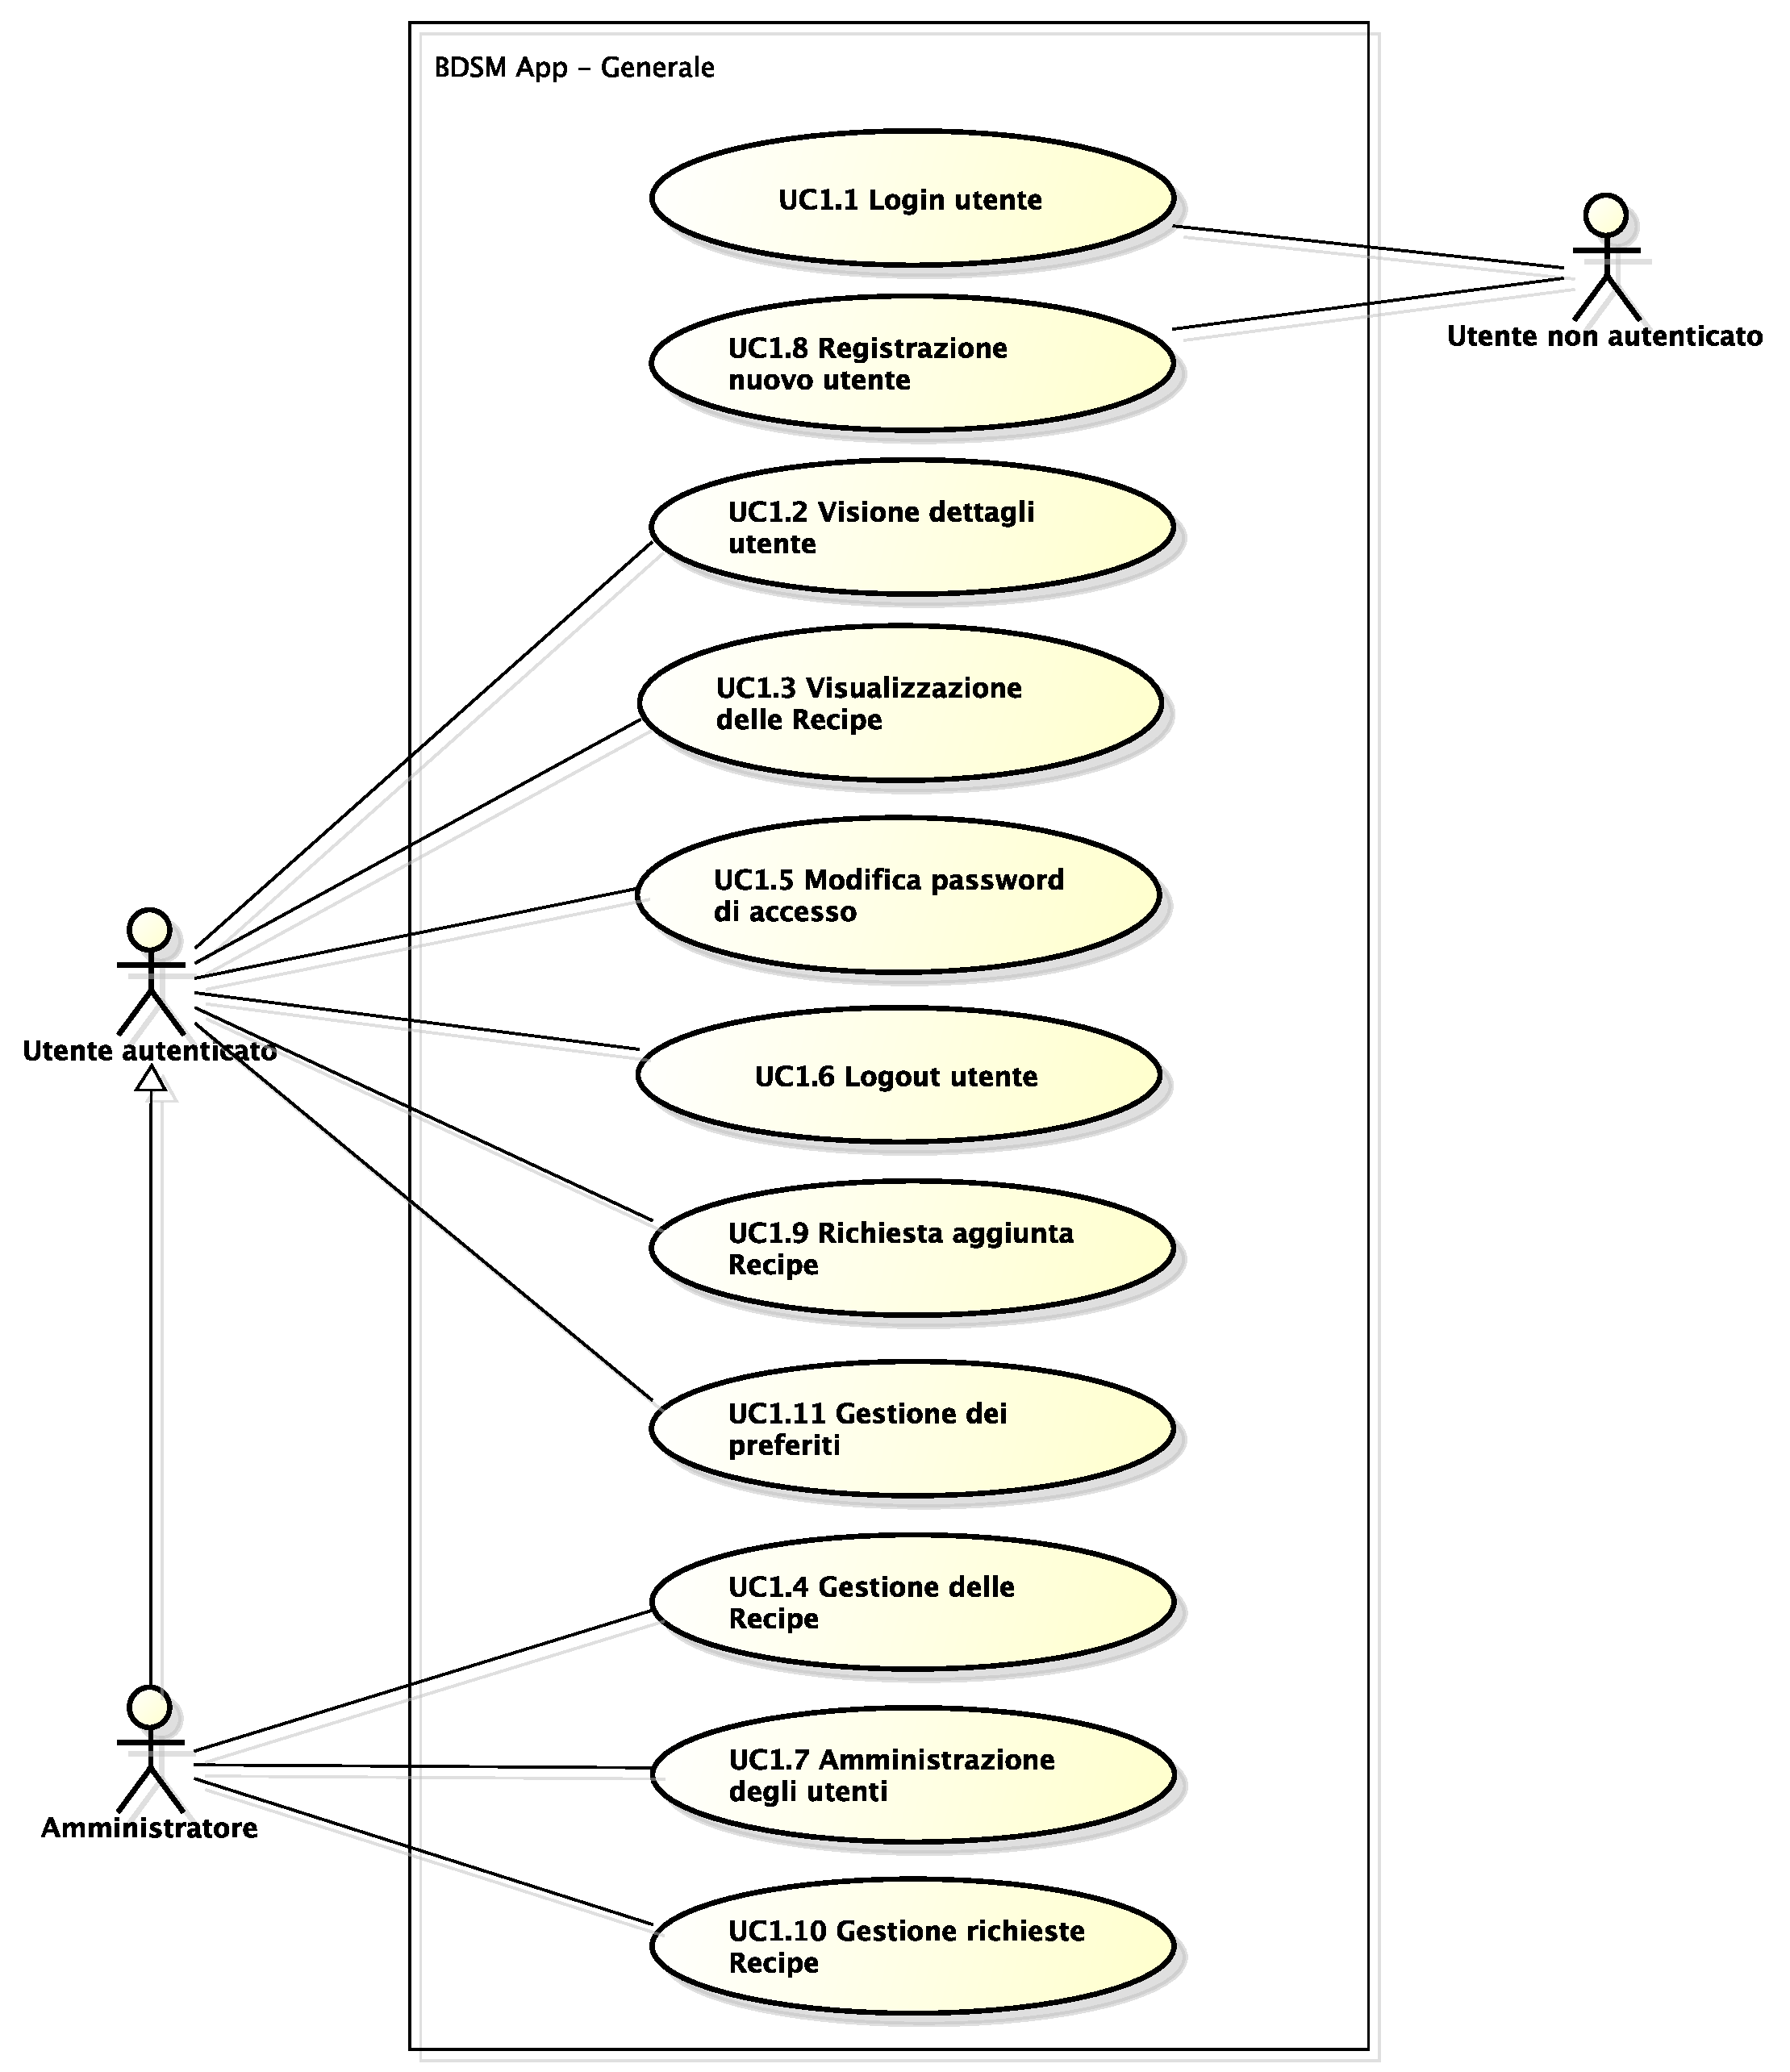
\includegraphics[scale=0.5]{./images/UC1.pdf}}
    \caption{Use Case 1 - Generale}
\end{figure}

\begin{itemize}

    \item \textbf{Attori Coinvolti:}
    \begin{itemize}
    
    	\item Utente sconosciuto: utente non autenticato che accede al servizio;
    	\item Utente autenticato: utente autenticato che ha avuto accesso al servizio;
    	\item Utente amministratore: utente autenticato che accesso al servizio e che dispone dei permessi per visualizzare tutte le aree;
	\end{itemize}
    \item \textbf{Descrizione:}
    dopo l'accesso al servizio:
    \begin{itemize}
    	\item un utente sconosciuto può autenticarsi, o se è al primo accesso al servizio può registrarsi per ottenere delle credenziali valide;
    	\item un utente autenticato può vedere statistiche, modificare la propria password, visualizzare, creare e modificare le proprie View;
  		\item un utente amministratore può fare tutte le operazioni di un utente autenticato, più ha la possibilità di eliminare un utente e tutte le sue View e modificarne i privilegi;
	\end{itemize}
    \item \textbf{Possibili Errori:}
    Viene visualizzato un messaggio di errore nel caso le informazioni di accesso inserite siano errate;

    \item \textbf{Postcondizione:}
    Il servizio ha erogato correttamente le funzionalità richieste dall'utente.

\end{itemize}

\subsection{UC 1.1: Login utente}

\begin{figure}[htbp]
    \centering
    \centerline{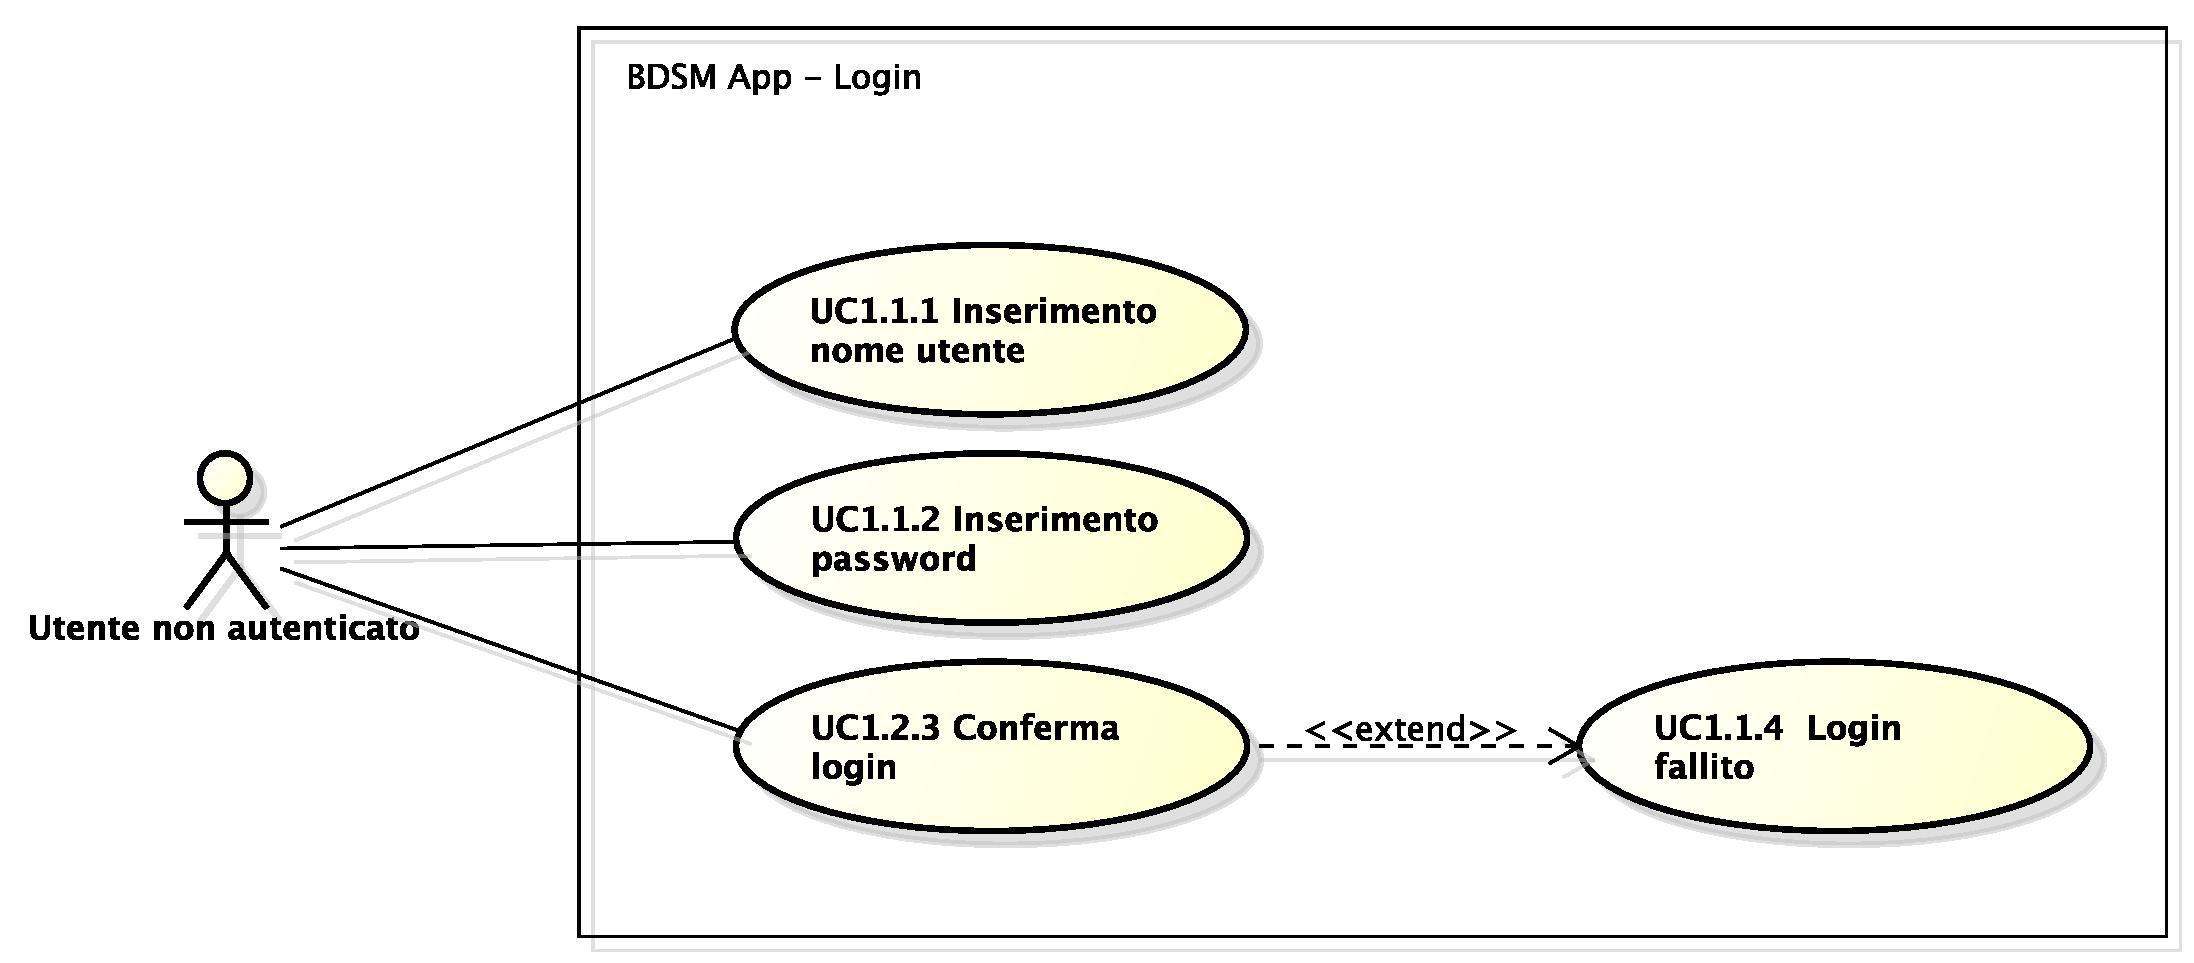
\includegraphics[scale=0.5]{./images/UC1_1.pdf}}
    \caption{Use Case 1.1 - Login utente}
\end{figure}


\begin{itemize}
    \item \textbf{Attori Coinvolti:}
    	utente non autenticato;
    \item \textbf{Precondizione:}
    	l'utente che accede alla pagina di accesso è sconosciuto al sistema;
    \item \textbf{Descrizione:}
    	l'utente può autenticarsi per poter accedere ai servizi offerti dalla piattaforma utilizzando la schermata di login;
    \item \textbf{Postcondizione:}
    	l'utente è riconosciuto dal sistema.
    \item \textbf{Possibili Errori:}
    	viene mostrato un messaggio di errore nel caso in cui i dati forniti siano errati;
    \item \textbf{Flusso principale degli eventi:}

    \begin{enumerate}
        \item inserimento username (UC 1.1.1);
        \item inserimento password (UC 1.1.2);
        \item pressione tasto login (UC 1.1.3);
    \end{enumerate}

\end{itemize}

\subsubsection{UC 1.1.1: Inserimento username}

\begin{itemize}
    \item \textbf{Attori:} utente non autenticato;
    \item \textbf{Descrizione:} l'utente non autenticato inserisce l'username;
    \item \textbf{Precondizione:} il sistema fornisce una schermata in cui è possibile inserire l’username;
    \item \textbf{Postcondizione:} il sistema ha l'informazione relativa all'username.
\end{itemize}

\subsubsection{UC 1.1.2: Inserimento password}

\begin{itemize}
    \item \textbf{Attori:} utente non autenticato;
    \item \textbf{Descrizione:} l'utente non autenticato inserisce la propria password personale;
    \item \textbf{Precondizione:} il sistema fornisce una schermata in cui è possibile inserire la password;
    \item \textbf{Postcondizione:} il sistema ha l'informazione relativa alla password inserita dall'utente.
\end{itemize}

\subsubsection{UC 1.1.3: Conferma login}

\begin{itemize}
    \item \textbf{Attori:} utente non autenticato;
    \item \textbf{Descrizione:} viene richiesto all'utente di confermare i dati inseriti con la pressione di un pulsante di conferma;
    \item \textbf{Precondizione:} il sistema fornisce un pulsante per confermare il login;
    \item \textbf{Postcondizione:} l'utente ha eseguito il login;
    \item \textbf{Estensioni:} Login fallita [UC 1.1.4].
\end{itemize}

\subsubsection{UC 1.1.4: Login fallita}

\begin{itemize}
    \item \textbf{Attori:} utente non autenticato;
    \item \textbf{Descrizione:} viene mostrato all'utente un messaggio di errore che riporta l'incorrettezza dei dati inseriti. Viene visualizzato un pulsante per tornare alla schermata di login;
    \item \textbf{Precondizione:} il sistema ha ricevuto una richiesta di accesso con dati errati;
    \item \textbf{Postcondizione:} l'utente ha preso atto del messaggio di errore.
\end{itemize}

\pagebreak

\subsection{UC 1.2: Visione informazioni e statistiche}

\begin{figure}[htbp]
    \centering
    \centerline{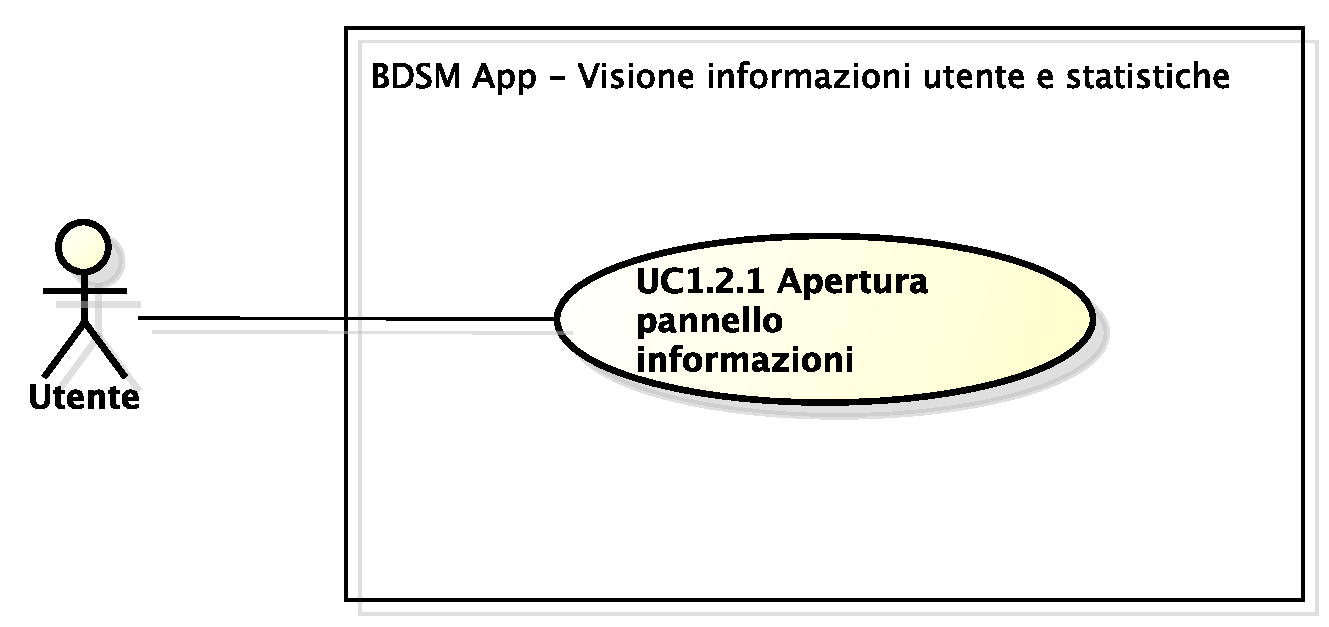
\includegraphics[scale=0.6]{./images/UC1_2.pdf}}
    \caption{Use Case 1.2 - Visione informazioni e statistiche}
\end{figure}

	\textbf{Attori Coinvolti:}
Utente autenticato: utente autenticato che ha acceduto al servizio
Utente amministratore autenticato: utente autenticato in grado di accedere a tutte le aree del servizio

	\textbf{Precondizione:}
L'utente deve aver fatto l'accesso nell'apposita pagina.

	\textbf{Descrizione:}
Gli utenti autenticati possono vedere una serie di informazioni relative alla loro attività, come la data dell’ultimo accesso effettuato e il numero di ricette e viste attive.

	\textbf{Postcondizione:}
Le informazioni richieste dall'utente sono state fornite

	\textbf{Possibili Errori:}
In caso di autenticazione scaduta verrà mostrata nuovamente la pagina di accesso.

\subsubsection{UC 1.2.1: Apertura pannello informazioni}

\begin{itemize}
    \item \textbf{Attori:} Utente
    \item \textbf{Descrizione:} Dalla Home Screen dell'utente è possibile, tramite un apposito menu, accedere al pannello informazioni e al pannello statistiche attinenti all'utente attualmente connesso.
    \item \textbf{Precondizione:} L'utente ha eseguito l'accesso al sistema.
    \item \textbf{Postcondizione:} L'utente ha visualizzato il contenuto del menù.
\end{itemize}

\subsubsection{UC 1.2.1.1: Visualizza informazioni utente}

\begin{itemize}
    \item \textbf{Attori:} Utente
    \item \textbf{Descrizione:} Selezionando il pulsante informazioni viene mostrata all'utente una pagina con il riepilogo dei sui dati, quali:
    \begin{enumerate}
        \item Il nome utente;
        \item L'indirizzo mail associato;
        \item La data dell'ultimo accesso effettuato;
    \end{enumerate}
    \item \textbf{Precondizione:} L'utente ha selezionato il pulsante di visualizzazione informazioni.
    \item \textbf{Postcondizione:} L'utente ha ottenuto le informazioni richieste.
\end{itemize}

\subsubsection{UC 1.2.1.2: Visualizza Statistiche utente}

\begin{itemize}
    \item \textbf{Attori:} Utente
    \item \textbf{Descrizione:} Selezionando il pulsante statistiche viene mostrata all'utente una pagina con il riepilogo delle sue statistiche, quali:
    \begin{enumerate}
        \item Numero di View attive;
        \item Numero di Recipe disponibili;
        \item Numero di accessi negli ultimi 30 giorni;
    \end{enumerate}
    \item \textbf{Precondizione:} L'utente ha selezionato il pulsante di visualizzazione statistiche.
    \item \textbf{Postcondizione:} L'utente ha ottenuto le informazioni richieste.
\end{itemize}

\clearpage


\subsection{UC 1.3: Gestione delle View}

\begin{figure}[!htbp]
    \centering
    \centerline{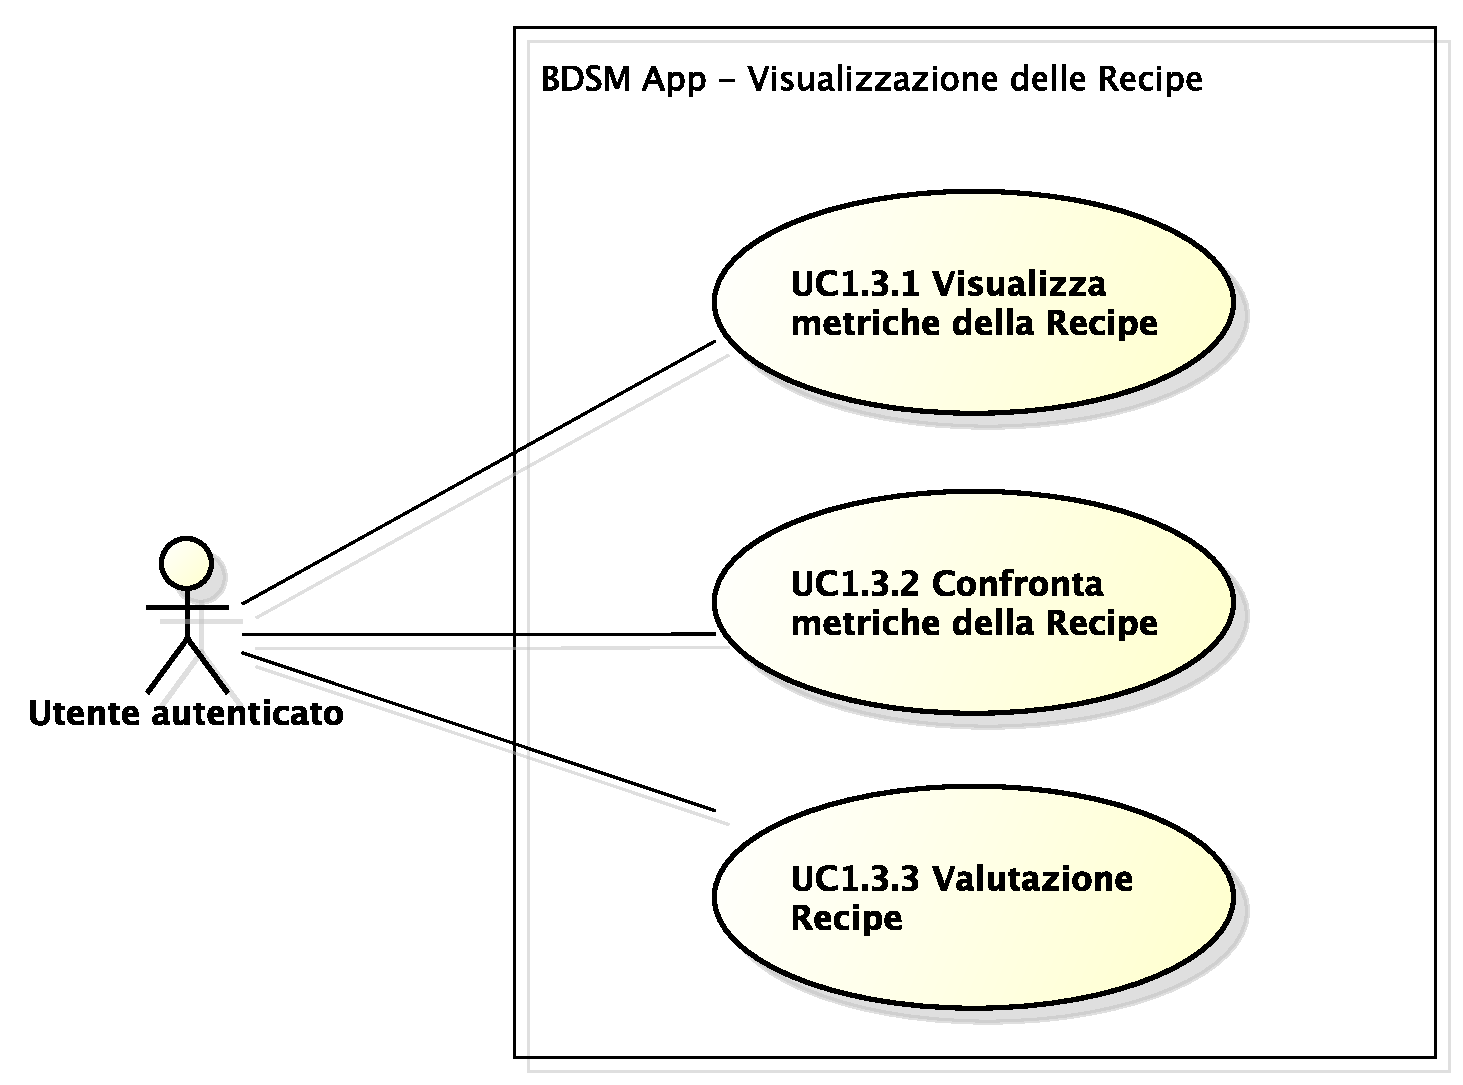
\includegraphics[scale=0.45]{./images/UC1_3.pdf}}
    \caption{Use Case 1.3 - Gestione delle View}
\end{figure}

\begin{itemize}
    \item \textbf{Attori Coinvolti:} Utente, Utente amministratore
    \item \textbf{Precondizione:} L’utente deve aver fatto l’accesso nell’apposita pagina.

    \item \textbf{Descrizione:} Gli utenti autenticati possono vedere in questa pagina le Views e i dati ad esse associati.
    Si rende disponibile per ciascuna View un pannello per modificarne i parametri.
    Si può creare una nuova View.
    Si può eliminare una View esistente.

    \item \textbf{Postcondizione:}
    Le informazioni richieste dall'utente sono state fornite
    Le impostazioni modificate sono state salvate nel sistema.
    Le informazioni aggiunte sono state salvate nel sistema.

    \item \textbf{Possibili Errori:}
    In caso di autenticazione scaduta verrà mostrata nuovamente la pagina di accesso.
\end{itemize}

\subsubsection{UC 1.3.1: Visualizza Views}

\begin{itemize}
    \item \textbf{Attori:} Utente
    \item \textbf{Descrizione:} Questa è la home screen dell'utente attualmente connesso. Qui è possibile visualizzare tutti o parte delle sue View e accedere ai menu di configurazione.
    \item \textbf{Precondizione:} L'utente ha effettuato il login oppure ha selezionato il pulsante per accedere a questa pagina.
    \item \textbf{Postcondizione:} L'utente viene reindirizzato alla home screen e visualizza le informazioni richieste.
\end{itemize}

\subsubsection{UC 1.3.1.1: Apertura elenco Views}

\begin{itemize}
    \item \textbf{Attori:} Utente
    \item \textbf{Descrizione:} Premendo sull'apposito pulsante è possibile far comparire a video l'elenco di tutte le Views utente.
    \item \textbf{Precondizione:} L'utente si trova nella home screen.
    \item \textbf{Postcondizione:} L'utente ha ottenuto l'elenco di tutte le sue Views
\end{itemize}

\subsubsection{UC 1.3.2: Aggiungi una View}

\begin{itemize}
    \item \textbf{Attori:} Utente
    \item \textbf{Descrizione:} Dalla home screen l'utente può aggiungere una nuova View premendo sull'apposito pulsante, compilando i dati richiesti e confermando l'operazione.
    \item \textbf{Precondizione:} L'utente si è autenticato e si trova nella home screen.
    \item \textbf{Postcondizione:} L'utente ha creato una nuovo View.
	\item \textbf{Possibili Errori:}
    Viene mostrato un messaggio di errore nel caso in cui i dati forniti siano errati.
    \item \textbf{Flusso principale degli eventi:}

    \begin{enumerate}
        \item apertura pannello (UC 1.3.2.1);
        \item inserimento parametri (UC 1.3.2.2);
        \item conferma creazione View (UC 1.3.2.3).
    \end{enumerate}

\end{itemize}

\subsubsection{UC 1.3.2.1: Apertura pannello inserimento nuova View}

\begin{itemize}
    \item \textbf{Attori:} Utente
    \item \textbf{Descrizione:} L'utente ha a disposizione un pulsante per aprire il pannello in cui inserire e selezionare i dati per la creazione di una nuova View.
    \item \textbf{Precondizione:} L'utente si trova nella home screen.
    \item \textbf{Postcondizione:} L'utente ha aperto il pannello di creazione di una nuova View.
\end{itemize}

\subsubsection{UC 1.3.2.2: Inserimento delle informazioni}

\begin{itemize}
    \item \textbf{Attori:} Utente
    \item \textbf{Descrizione:} L'utente può inserire il nome e i parametri obbligatori e facoltativi relativi ad una nuova View.
    \item \textbf{Precondizione:} L'utente ha aperto il pannello di inserimento nuova View.
    \item \textbf{Postcondizione:} L'utente ha inserito le informazioni richieste.
\end{itemize}

\subsubsection{UC 1.3.2.3: Conferma delle informazioni inserite}

\begin{itemize}
    \item \textbf{Attori:} Utente
    \item \textbf{Descrizione:} L'utente è tenuto a confermare i parametri inseriti nel pannello di creazione di una nuova View prima di poter utilizzare il grafico associato.
    \item \textbf{Precondizione:} L'utente ha inserito almeno tutti i parametri obbligatori richiesti.
    \item \textbf{Postcondizione:} L'utente ha confermato i parametri inseriti e la View è stata salvata nel sistema.
    \item \textbf{Possibili Errori:} L'utente ha inserito delle informazioni errate o non ha rispettato i vincoli del sistema.
\end{itemize}

\subsubsection{UC 1.3.3: Errore nella Creazione di nuova View}

\begin{itemize}
    \item \textbf{Attori:} Utente
    \item \textbf{Descrizione:} In caso i dati inseriti non rispettino i vincoli del sistema oppure se si verifica un errore lato server viene visualizzata questa pagina di errore con i dettagli dei vincoli non rispettati o una breve descrizione dell'errore rilevato.
    \item \textbf{Precondizione:} L'utente ha inserito dei dati che non rispettano i vincoli dl sistema. Il server ha sollevato un'eccezione durante il salvataggio dei dati.
    \item \textbf{Postcondizione:} Nessuna modifica richiesta è stata salvata nel sistema.
\end{itemize}

\subsubsection{UC 1.3.4: Modifica una View}

\begin{itemize}
    \item \textbf{Attori:} Utente
    \item \textbf{Descrizione:} L'utente può modificare i parametri associati ad una specifica View.
    \item \textbf{Precondizione:} La View è stata creata ed è disponibile nell'elenco Views dell'utente.
    \item \textbf{Postcondizione:} I parametri relativi alla View sono stati modificati.

	\item \textbf{Possibili Errori:}
    Viene mostrato un messaggio di errore nel caso in cui i dati forniti siano errati.
    \item \textbf{Flusso principale degli eventi:}

    \begin{enumerate}
        \item selezione di una View (UC 1.3.4.1);
        \item selezione tasto modifica (UC 1.3.4.2);
        \item inserimento nuovi parametri (UC 1.3.4.3);
        \item conferma nuovi parametri (UC 1.3.4.4).
    \end{enumerate}

\end{itemize}

\subsubsection{UC 1.3.4.1: Selezione di una View}

\begin{itemize}
    \item \textbf{Attori:} Utente
    \item \textbf{Descrizione:} L'utente deve selezionare la View desiderata dall'elenco delle View per poterla visualizzare e modificare.
    \item \textbf{Precondizione:} L'utente si trova nel suo elenco delle View.
    \item \textbf{Postcondizione:} L'utente ha selezionato e visualizzato la View desiderata.
\end{itemize}

\subsubsection{UC 1.3.4.2: Apertura pannello modifica View}

\begin{itemize}
    \item \textbf{Attori:} Utente
    \item \textbf{Descrizione:} L'utente può selezionare il pulsante modifica dal pannello della View attualmente visualizzata per modificarne i parametri.
    \item \textbf{Precondizione:} L'utente ha visualizzato correttamente una View.
    \item \textbf{Postcondizione:} L'utente ha aperto il pannello modifica View.
\end{itemize}

\subsubsection{UC 1.3.4.3: Inserimento dei parametri}

\begin{itemize}
    \item \textbf{Attori:} Utente
    \item \textbf{Descrizione:} L'utente può inserire i nuovi parametri della View aggiungendoli a quelli esistenti oppure sovrascrivendoli.
    \item \textbf{Precondizione:} L'utente ha visualizzato il pannello modifica View.
    \item \textbf{Postcondizione:} L'utente ha inserito i nuovi parametri.
\end{itemize}

\subsubsection{UC 1.3.4.4: Conferma dei parametri inseriti}

\begin{itemize}
    \item \textbf{Attori:} Utente
    \item \textbf{Descrizione:} L'utente deve confermare i parametri inseriti perima che questi siano attivi.
    \item \textbf{Precondizione:} L'utente ha inserito i parametri desiderati nei campi del pannello di modifica View.
    \item \textbf{Postcondizione:} I nuovi parametri sono stati memorizzati nel sistema e sono ora attivi.
\end{itemize}

\subsubsection{UC 1.3.5: Errore nella modifica della View}

\begin{itemize}
    \item \textbf{Attori:} Utente
    \item \textbf{Descrizione:} L'utente visualizza una schermata di errore con i parametri che ha inserito non conformi ai vincoli di sistema.
    \item \textbf{Precondizione:} L'utente ha inserito dei parametri non validi.
    \item \textbf{Postcondizione:} L'utente ha visualizzato il messaggio di errore e ha preso atto dei parametri inseriti non conformi ai vincoli di sistema.
\end{itemize}

\subsubsection{UC 1.3.6: Eliminazione di una View}

\begin{itemize}
    \item \textbf{Attori:} Utente
    \item \textbf{Descrizione:} L'utente può eliminare una View precedentemente creata.
    \item \textbf{Precondizione:} L'utente ha creato almeno una View e questa è visualizzata nell'elenco delle sue View.
    \item \textbf{Postcondizione:} L'utente ha cancellato una View dal suo profilo.
    \item \textbf{Flusso principale degli eventi:}

    \begin{enumerate}
        \item selezione di una View (UC 1.3.6.1);
        \item selezione pulsante elimina (UC 1.3.6.2);
        \item conferma eliminazione (UC 1.3.6.3).
    \end{enumerate}

\end{itemize}

\subsubsection{UC 1.3.6.1: Selezione di una View}

\begin{itemize}
    \item \textbf{Attori:} Utente
    \item \textbf{Descrizione:} L'utente deve selezionare la View desiderata dall'elenco delle View per poterla visualizzare e modificare.
    \item \textbf{Precondizione:} L'utente si trova nel suo elenco delle View.
    \item \textbf{Postcondizione:} L'utente ha selezionato e visualizzato la View desiderata.
\end{itemize}

\subsubsection{UC 1.3.6.2: Eliminazione di una View}

\begin{itemize}
    \item \textbf{Attori:} Utente
    \item \textbf{Descrizione:} L'utente può selezionare il pulsante Elimina View dalla View correntemente visualizzata.
    \item \textbf{Precondizione:} L'utente ha visualizzato correttamente una delle sue View.
    \item \textbf{Postcondizione:} L'utente ha selezionato il pulsante Elimina View.
\end{itemize}

\subsubsection{UC 1.3.6.3: Conferma eliminazione di una View}

\begin{itemize}
    \item \textbf{Attori:} Utente
    \item \textbf{Descrizione:} L'utente deve confermare l'eliminazione delle View selezionando il pulsante di conferma sul messaggio di conferma eliminazione View.
    \item \textbf{Precondizione:} L'utente ha selezionato il pulsante di eliminazione di una View.
    \item \textbf{Postcondizione:} L'utente ha confermato l'eliminazione e la View è stata eliminata dal sistema.
\end{itemize}

\clearpage


\subsection{UC 1.4: Gestione delle Recipe}

\begin{figure}[!ht]
    \centering
    \centerline{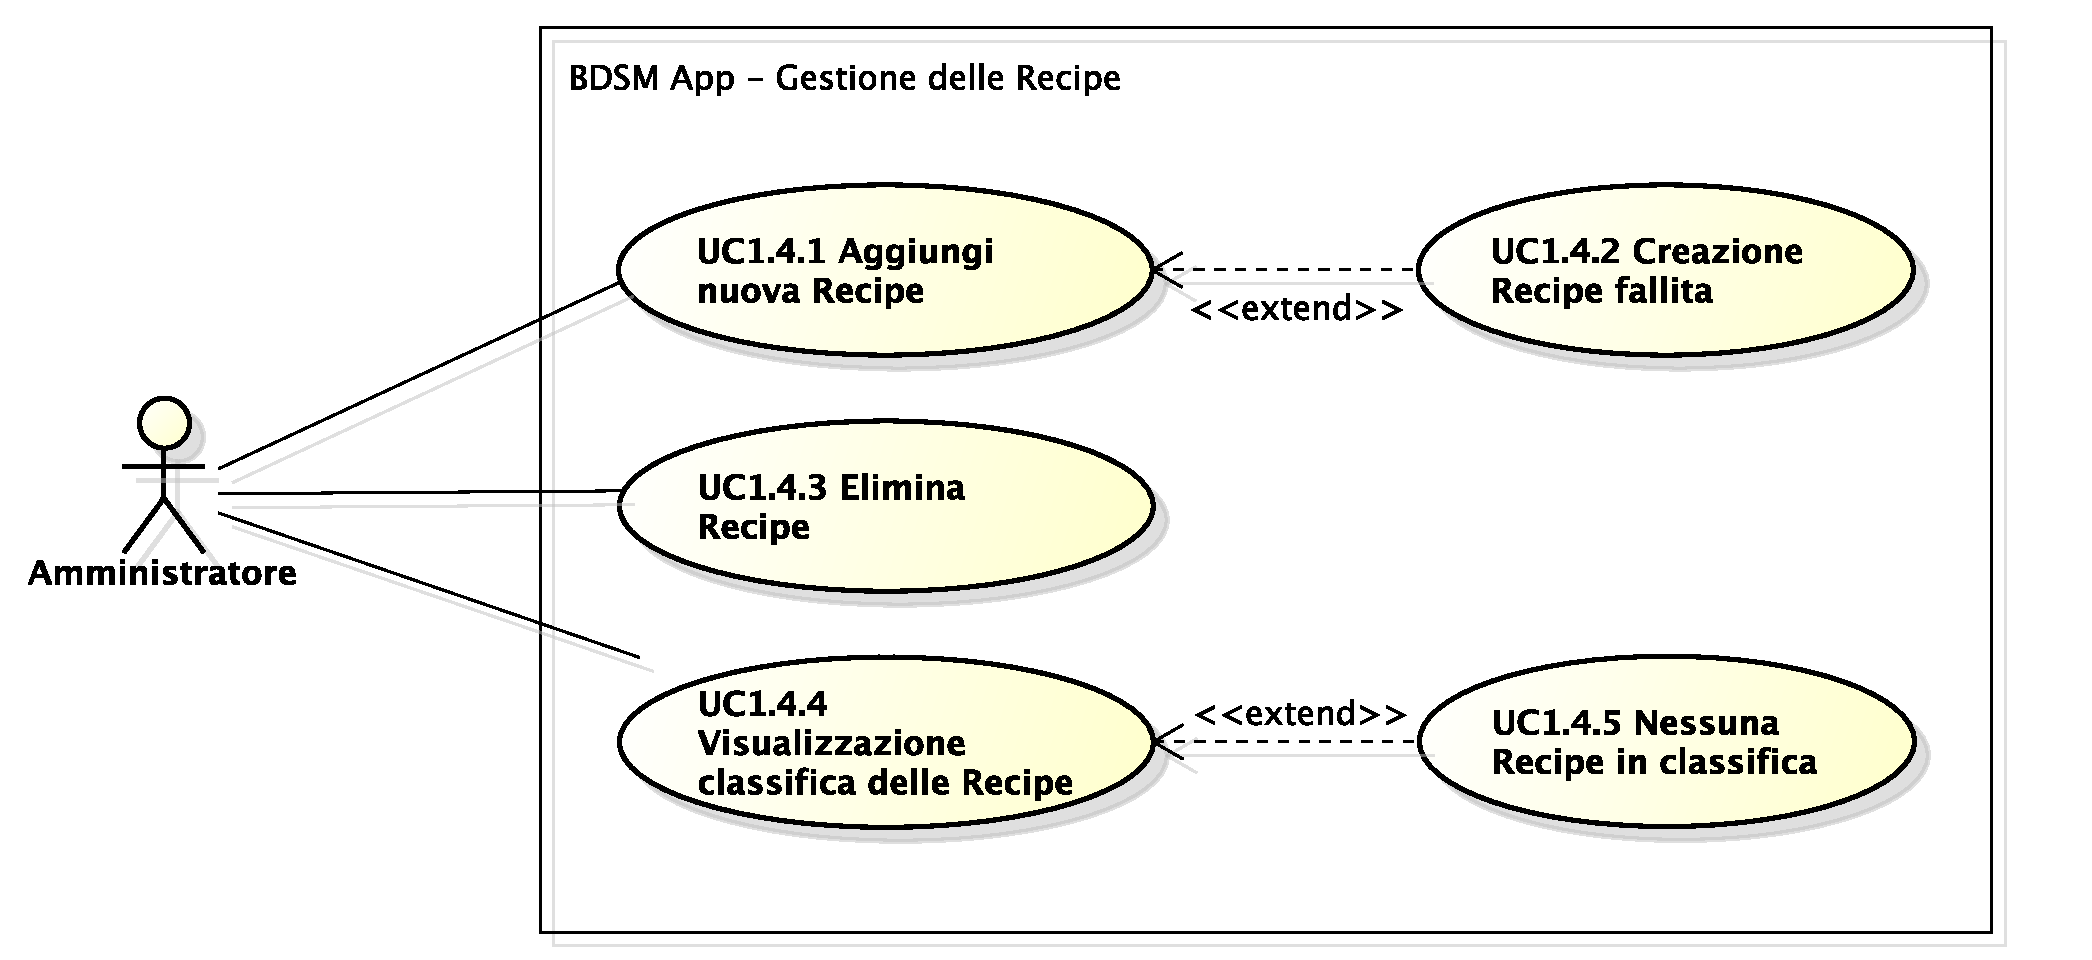
\includegraphics[scale=0.5]{./images/UC1_4.pdf}}
    \caption{Use Case 1.4 - Gestione delle Recipe}
\end{figure}

\begin{itemize}
    \item \textbf{Attori Coinvolti:} Utente Amministratore

    \item \textbf{Precondizione:} L'utente deve aver fatto l'accesso nell'apposita pagina.

    \item \textbf{Descrizione:} Gli utenti amministratori possono vedere in questa pagina le ricette e i dati ad esse associati. Essi possono creare oppure eliminare una Recipe.

    \item \textbf{Postcondizione:} Le informazioni richieste dall'utente sono state fornite.
    Le Recipe eliminate sono state cancellate dal sistema.
    Le Recipe aggiunte sono state salvate nel sistema.

    \item \textbf{Possibili Errori:} In caso di autenticazione scaduta verrà mostrata nuovamente la pagina di accesso.
\end{itemize}

\subsubsection{UC 1.4.1: Visualizza Recipes}

\begin{itemize}
    \item \textbf{Attori:} Utente Amministratore
    \item \textbf{Descrizione:} L'utente amministratore può visualizzare l'elenco di tutte le Recipe salvate nel sistema selezionando l'apposito pulsante nella sua home screen.
    \item \textbf{Precondizione:} L'utente amministratore ha effettutao l'accesso al sistema e si trova nella sua home screen.
    \item \textbf{Postcondizione:} L'utente ha visualizzato correttamente l'elenco delle Recipes salvate nel sistema.
\end{itemize}

\subsubsection{UC 1.4.2: Aggiungi una nuova Recipe}

\begin{itemize}
    \item \textbf{Attori:} Utente Amministratore
    \item \textbf{Descrizione:} L'utente amministratore può aggiungere una nuova Recipe al sistema.
    \item \textbf{Precondizione:} L'utente amministratore ha visualizzato l'elenco delle Recipes salvate nel sistema.
    \item \textbf{Postcondizione:} L'utente amministratore ha salvato una nuova Recipe nel sistema.
	\item \textbf{Possibili Errori:}
    Viene mostrato un messaggio di errore nel caso in cui i dati forniti siano errati.
    \item \textbf{Flusso principale degli eventi:}

    \begin{enumerate}
        \item apertura elenco Recipes (UC 1.4.2.1);
        \item apertura pannello inserimento (UC 1.4.2.2);
        \item inserimento parametri (UC 1.4.2.3);
        \item conferma parametri inseriti (UC 1.4.2.4).
    \end{enumerate}

\end{itemize}

\subsubsection{UC 1.4.2.1: Apertura elenco Recipes}

\begin{itemize}
    \item \textbf{Attori:} Utente Amministratore
    \item \textbf{Descrizione:} L'utente amministratore può visualizzare l'elenco delle Recipes salvate nel sistema premendo l'apposito pulsante nella sua Home Screen.
    \item \textbf{Precondizione:} L'utente amministratore ha effettuato l'accesso al sistema.
    \item \textbf{Postcondizione:} L'utente amministratore ha visualizzato correttamente l'elenco delle Recipes.
\end{itemize}

\subsubsection{UC 1.4.2.2: Apertura pannello inserimento nuova Recipe}

\begin{itemize}
    \item \textbf{Attori:} Utente Amministratore
    \item \textbf{Descrizione:} L'utente amministratore può selezionare il pulsante di inserimento di una nuova Recipe dall'elenco delle Recipes.
    \item \textbf{Precondizione:} L'utente amministratore ha visualizzato l'elenco delle Recipes.
    \item \textbf{Postcondizione:} L'utente amministratore ha visualizzato il pannello di inserimento nuova Recipe.
\end{itemize}

\subsubsection{UC 1.4.2.3: Inserimento dei parametri}

\begin{itemize}
    \item \textbf{Attori:} Utente Amministratore
    \item \textbf{Descrizione:} L'utente amministratore può inserire il nome ed i parametri per la nuova Recipe nel pannello di inserimento nuova Recipe.
    \item \textbf{Precondizione:} L'utente amministratore ha selezionato il pulsante per l'inseriemnto di una nuova Recipe.
    \item \textbf{Postcondizione:} L'utente ha inserito tutti i parametri richiesti dal sistema.
\end{itemize}

\subsubsection{UC 1.4.2.4: Conferma dei parametri inserite}

\begin{itemize}
    \item \textbf{Attori:} Utente Amministratore
    \item \textbf{Descrizione:} L'utente amministratore deve confermare i parametri inseriti prima che questi siano attivi nel sistema.
    \item \textbf{Precondizione:} L'utente ha inserito almeno tutti i parametri obbligatori richiesti dal sistema.
    \item \textbf{Postcondizione:} L'utente amministratore ha confermato i parametri inseriti.
\end{itemize}

\subsubsection{UC 1.4.3: Errore nell'inserimento di una nuova Recipe}

\begin{itemize}
    \item \textbf{Attori:} Utente Amministratore
    \item \textbf{Descrizione:} L'utente amministratore ha inserito dei parmetri che non rispettano i vincoli di sistema durante l'inserimento di una nuova Recipe.
    \item \textbf{Precondizione:} L'utente amministratore ha selezionato il pulsante di conferma per la creazione di una nuova Recipe.
    \item \textbf{Postcondizione:} L'utente amministratore ha visualizzato un messaggio di errore contenente l'elenco dei parametri inseriti non corretti oppure contenente l'eccezione sollevata dal sistema durante il salvataggio della nuova Recipe.
\end{itemize}

\subsubsection{UC 1.4.4: Eliminazione di una Recipe}

\begin{itemize}
    \item \textbf{Attori Coinvolti:}
    Utente Amministratore

    \item \textbf{Precondizione:}
    L'utente amministratore deve aver visualizzato la schermata di gestione delle Recipes.

    \item \textbf{Descrizione}:
    L'utente amministratore può eliminare una Recipe e tutti i dati ad essa associati.
    Si possono eliminare solo le Recipe non più utilizzate in una o più viste proprie o di un altro utente.

    \item \textbf{Postcondizione:}
    Le informazioni richieste dall'utente sono state fornite.
    La Recipe desiderata e tutti i dati ad essa associati sono stati eliminati dal sistema.

    \item \textbf{Possibili Errori:}
    In caso di autenticazione scaduta verrà mostrata nuovamente la pagina di accesso.
    In caso di Recipe in uso o in fase di aggiornamento a causa di una schedulazione viene visualizzato un messaggio di errore e nessun dato viene alterato o cancellato.
	\item \textbf{Possibili Errori:}
    Viene mostrato un messaggio di errore nel caso in cui i dati forniti siano errati.
    \item \textbf{Flusso principale degli eventi:}

    \begin{enumerate}
        \item apertura elenco Recipes (UC 1.4.4.1);
        \item eleminazione di una Recipe (UC 1.4.4.2);
        \item conferma eliminazione Recipe (UC 1.4.4.3).
    \end{enumerate}

\end{itemize}

\subsubsection{UC 1.4.4.1: Apertura elenco Recipes}

\begin{itemize}
    \item \textbf{Attori:} Utente Amministratore
    \item \textbf{Descrizione:} L'utente amministratore può visualizzare l'elenco delle Recipes salvate nel sistema premendo l'apposito pulsante nella sua Home Screen.
    \item \textbf{Precondizione:} L'utente amministratore ha effettuato l'accesso al sistema.
    \item \textbf{Postcondizione:} L'utente amministratore ha visualizzato correttamente l'elenco delle Recipes.
\end{itemize}

\subsubsection{UC 1.4.4.2: Eliminazione di una Recipe}

\begin{itemize}
    \item \textbf{Attori:} Utente Amministratore
    \item \textbf{Descrizione:} L'utente amministratore può selezionare il pulsante di eliminazione su una Recipe nell'elenco delle Recipes.
    \item \textbf{Precondizione:} L'utente amministratore ha visualizzato l'elenco delle Recipes.
    \item \textbf{Postcondizione:} L'utente amministratore ha selezionato il pulsante di eliminazione di una Recipe.
\end{itemize}
\subsubsection{UC 1.4.4.3: Conferma eliminazione di una Recipe}

\begin{itemize}
    \item \textbf{Attori:} Utente Amministratore
    \item \textbf{Descrizione:} L'utente amministratore deve confermare la volontà di eliminare la Recipe selezionando il pulsante di conferma eliminazione.
    \item \textbf{Precondizione:} L'utente amministratore ha selezionato il pusante elimina su una Recipe.
    \item \textbf{Postcondizione:} L'utente amministratore ha confermat l'eliminazione della Recipe e questa è stata cancellata dal sistema insieme a tutti i dati ad essa associati.
\end{itemize}

\clearpage


\subsection{UC 1.5: Modifica Password di accesso}

\begin{figure}[!htbp]
    \centering
    \centerline{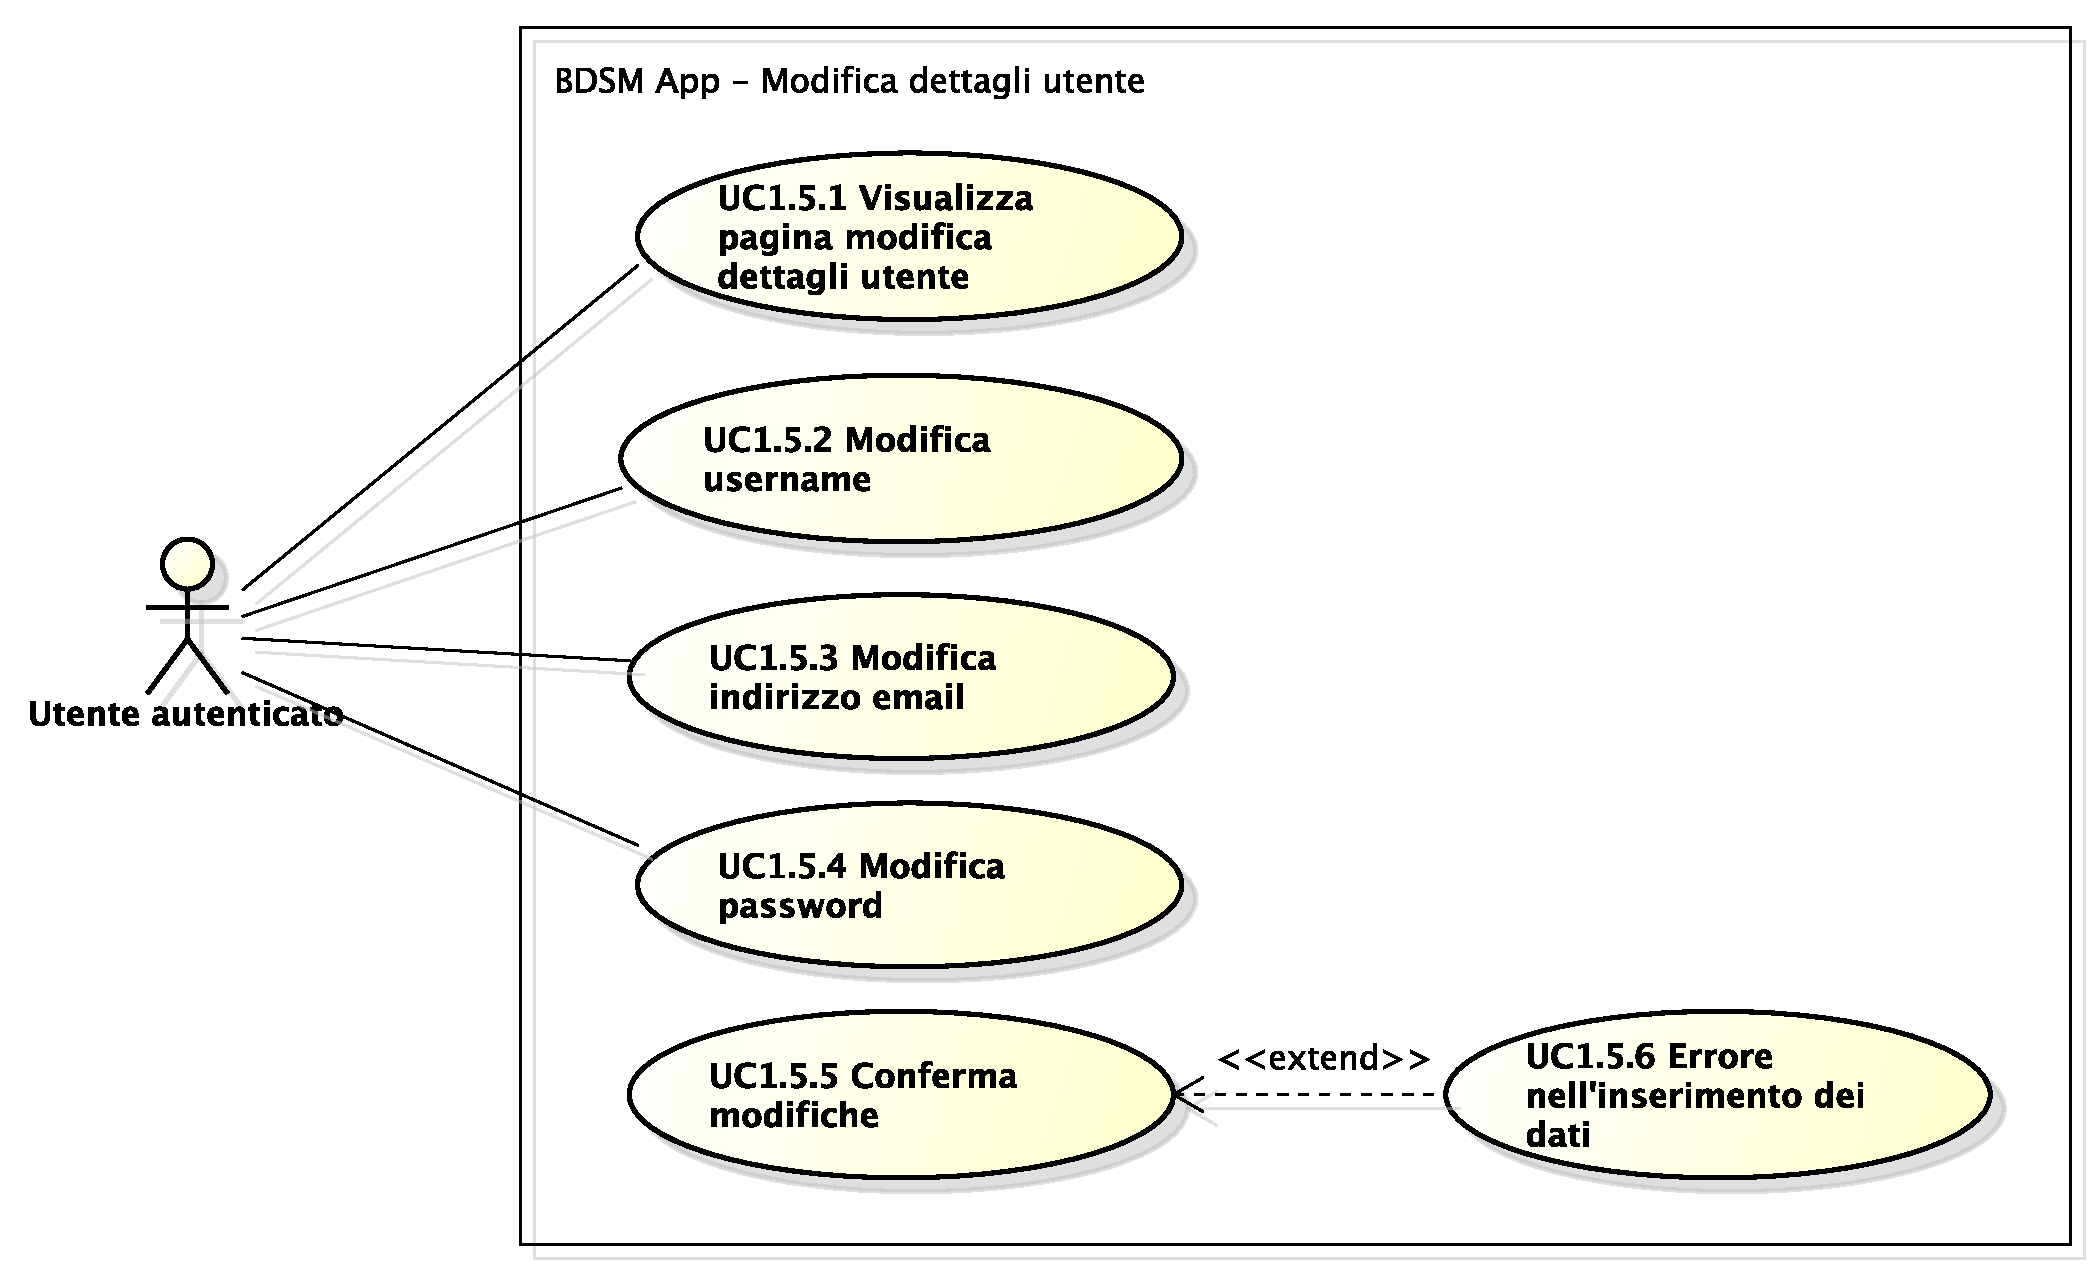
\includegraphics[scale=0.4]{./images/UC1_5.pdf}}
    \caption{Use Case 1.5 - Modifica password di accesso}
\end{figure}

\begin{itemize}
    \item \textbf{Attori Coinvolti:} Utente
    \item \textbf{Precondizione:} L'utente dispone di una password di accesso valida, risulta autenticato al servizio e si trova nella sua Home Screen.
    \item \textbf{Descrizione:} L'utente può cambiare la password attualmente in uso selezionando il pulsante di cambio password sulla sua Home Screen.
    \item \textbf{Postcondizione:} La nuova password per l'utente è attiva, la vecchia password non è più valida.
    \item \textbf{Possibili Errori:} Messaggio di errore in caso di informazioni inserite errate oppure la nuova password non soddisfa i criteri di sistema indicati (UC 1.5.4).

    \begin{enumerate}
        \item inserimento nuova password (UC 1.5.1);
        \item inserimento nuova password per conferma (UC 1.5.2);
        \item conferma cmbio password (UC 1.5.3).
    \end{enumerate}

\end{itemize}

\subsubsection{UC 1.5.1: Inserimento di una nuova password}

\begin{itemize}
    \item \textbf{Attori:} Utente
    \item \textbf{Descrizione:} L'utente può inserire la nuova password nel pannello di cambio password.
    \item \textbf{Precondizione:} L'utente ha selezionato il pulsante di cambio password nella sua Home Screen.
    \item \textbf{Postcondizione:} L'utente ha inserito la nuova password.
\end{itemize}

\subsubsection{UC 1.5.2: Conferma inserimento password }

\begin{itemize}
    \item \textbf{Attori:} Utente
    \item \textbf{Descrizione:} L'utente deve inserire nuovamente la nuova password per verificare di non aver fatto errori di battitura.
    \item \textbf{Precondizione:} L'utente ha inserito la nuova password.
    \item \textbf{Postcondizione:} L'utente ha inserito per la seconda volta la nuova password.
\end{itemize}

\subsubsection{UC 1.5.3: Inserimento vecchia password}

\begin{itemize}
    \item \textbf{Attori:} Utente
    \item \textbf{Descrizione:} L'utente deve inserire la vecchia password per completare il cambio password.
    \item \textbf{Precondizione:} L'utente ha inserito la nuova password due volte negli appositi campi.
    \item \textbf{Postcondizione:} L'utente ha confermato l'operazione e la nuova password è ora attiva.
\end{itemize}

\subsubsection{UC 1.5.4: Conferma operazione}

\begin{itemize}
    \item \textbf{Attori:} Utente
    \item \textbf{Descrizione:} L'utente deve confermare la volontà di sostituire la password di accesso con quella nuova selezionando il pulsante di conferma.
    \item \textbf{Precondizione:} L'utente ha inserito due volte la nuova password ed una la vecchia negli appositi campi.
    \item \textbf{Postcondizione:} L'utente ha confermato l'operazione e la nuova password è ora attiva.
\end{itemize}

\subsubsection{UC 1.5.5: Password inserita non conforme alle regole}

\begin{itemize}
    \item \textbf{Attori:} Utente
    \item \textbf{Descrizione:} L'utente può aver inserito una password che non soddisfa i vincoli di sistema indicati nel pannello di cambio password.
    \item \textbf{Precondizione:} L'utente ha selezionato il pulsante di conferma del cambio password.
    \item \textbf{Postcondizione:} L'utente ha visualizzato un messaggio di errore con i dettagli dei vincoli non soddisfatti.
\end{itemize}

\clearpage


\subsection{UC 1.6: Logout}

\begin{figure}[htbp]
    \centering
    \centerline{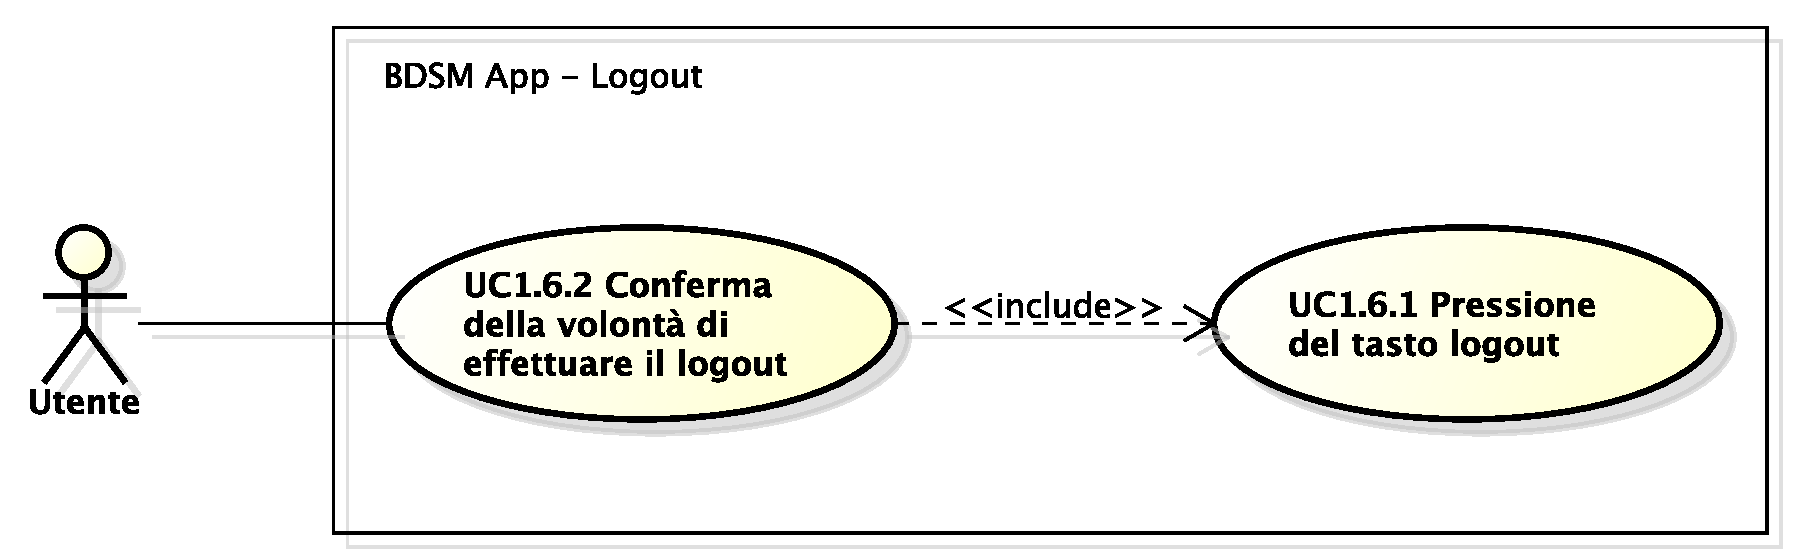
\includegraphics[scale=0.5]{./images/UC1_6.pdf}}
    \caption{Use Case 1.6 - Logout}
\end{figure}

\begin{itemize}
    \item \textbf{Attori Coinvolti:} Utente, Utente amministratore
    \item {Precondizione:} L'utente risulta autenticato al servizio.
    \item \textbf{Descrizione:} L'utente può terminare la sessione di lavoro e liberare la postazione per un altro utente. Questa operazione può essere eseguita premendo il pulsante Logout nella Home Screen.
    \item \textbf{Postcondizione:} La sessione di lavoro è terminata. Viene mostrata la schermata di Login.
    \item \textbf{Possibili Errori:} La sessione è scaduta. Non è quindi possibile eseguire questa operazione.
\end{itemize}

\subsubsection{UC 1.6.1: Pressione tasto logout}

\begin{itemize}
    \item \textbf{Attori:} Utente
    \item \textbf{Descrizione:} L'utente può effettuare il logout selezionando l'apposito pulsante nella sua Home Screen
    \item \textbf{Precondizione:} L'utente ha effettuato l'accesso al servizio e si trova nella Home Screen.
    \item \textbf{Postcondizione:} L'utente visualizza il pannello di conferma logout.
\end{itemize}

\subsubsection{UC 1.6.2: Conferma della volontà di fare logout}

\begin{itemize}
    \item \textbf{Attori:} Utente
    \item \textbf{Descrizione:} Prima di terminare la sessione di lavoro l'utente deve confermare la volontà di farlo selezionando il pulsante di conferma sul pannello di logout.
    \item \textbf{Precondizione:} L'utente ha selezionato il pulsante di logout nella Home Screen.
    \item \textbf{Postcondizione:} L'utente ha confermato la volontà di fare logout e la sessione è terminata. Viene visualizzata la schermata di login.
\end{itemize}

\clearpage


\subsection{UC 1.7: Amministrazione degli utenti}

\begin{figure}[!htbp]
    \centering
    \centerline{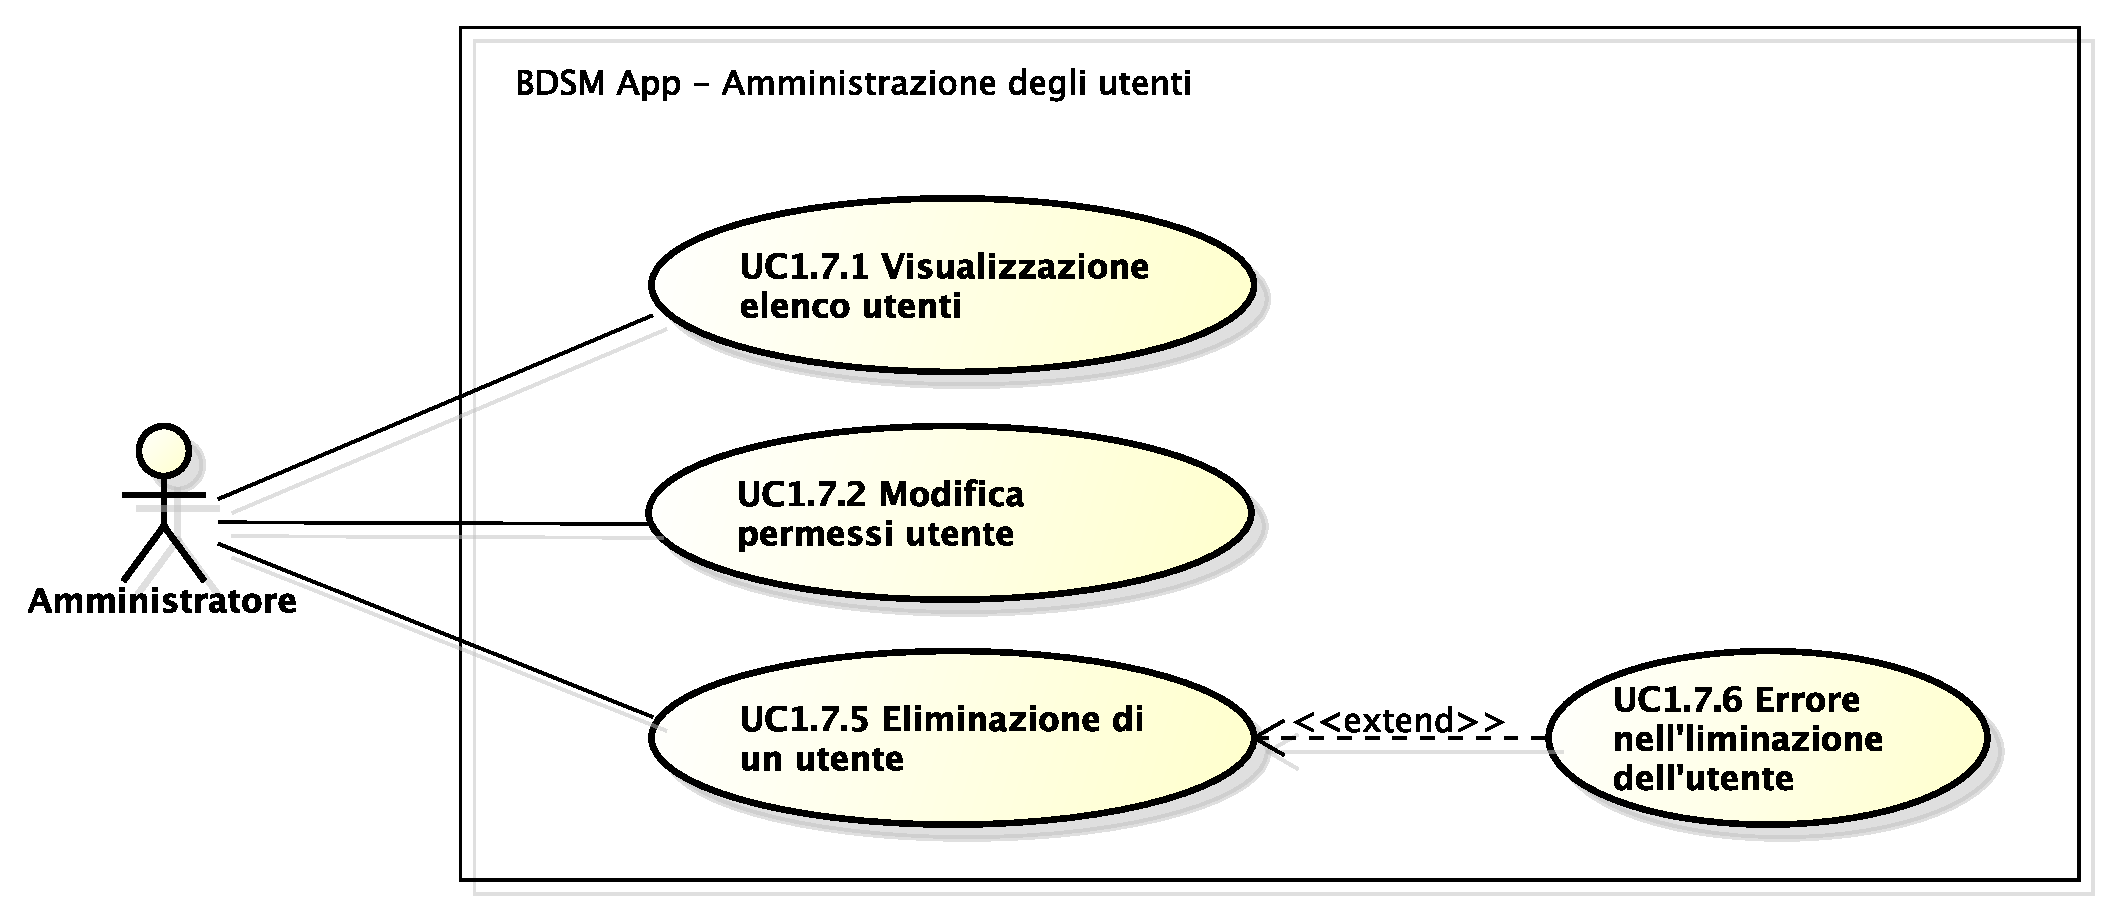
\includegraphics[scale=0.45]{./images/UC1_7.pdf}}
    \caption{Use Case 1.7 - Amministrazioni degli utenti}
\end{figure}

\begin{itemize}
    \item \textbf{Attori:} Utente amministratore
    \item \textbf{Descrizione:} L'utente amministratore può promuovere o diminuire i permessi di accesso di un altro utente. Può anche eliminare definitivamente un utente e tutte le sue Views.
    \item \textbf{Precondizione:} L'utente amministratore ha effettuato l'accesso al sistema.
    \item \textbf{Postcondizione:} Il sistema ha eseguito le operazioni richieste.
\end{itemize}

\subsubsection{UC 1.7.1: Visualizzazione elenco utenti}

\begin{itemize}
    \item \textbf{Attori:} Utente amministratore
    \item \textbf{Descrizione:} L'utente amministratore può visualizzare l'elenco di tutti gli utenti salvati nel sistema selezionando l'apposito pulsante nella sua Home Screen.
    \item \textbf{Precondizione:} L'utente amministratore ha effettuato l'accesso al sistema e si trova nella sua Home Screen.
    \item \textbf{Postcondizione:} L'utente amministratore ha visualizzato l'elenco degli utenti.
\end{itemize}

\subsubsection{UC 1.7.2: Modifica permessi utente}

\begin{itemize}
    \item \textbf{Attori:} Utente amministratore
    \item \textbf{Descrizione:} L'utente amministratore può cambiare i permessi di accesso al sistema ad un utente diverso da se stesso.
    \item \textbf{Precondizione:} L'utente amministratore ha eseguito l'accesso.
    \item \textbf{Postcondizione:} L'utente amministratore ha modificato i permessi ad un utente.
    \item \textbf{Possibili Errori:}
    Viene mostrato un messaggio di errore nel caso in cui i dati forniti siano errati.
    \item \textbf{Flusso principale degli eventi:}

    \begin{enumerate}
        \item apertura elenco utenti (UC 1.7.2.1);
        \item apertura pannello modifica (UC 1.7.2.2);
        \item inserimento dei nuovi parametri (UC 1.7.2.3);
        \item conferma parametri inseriti (UC 1.7.2.4)
    \end{enumerate}

\end{itemize}

\subsubsection{UC 1.7.2.1: Apertura elenco utenti}

\begin{itemize}
    \item \textbf{Attori:} Utente amministratore
    \item \textbf{Descrizione:} L'utente amministratore può visualizzare l'elenco di tutti gli utenti salvati nel sistema selezionando l'apposito pulsante nella sua Home Screen.
    \item \textbf{Precondizione:} L'utente amministratore ha effettuato l'accesso al sistema e si trova nella sua Home Screen.
    \item \textbf{Postcondizione:} L'utente amministratore ha visualizzato l'elenco degli utenti.
\end{itemize}

\subsubsection{UC 1.7.2.2: Selezione modifica su un utente}

\begin{itemize}
    \item \textbf{Attori:} Utente amministratore
    \item \textbf{Descrizione:} L'utente amministratore può cambiare i permessi di accesso ad un utente premendo l'apposito pulsante di fianco al suo username nell'elenco utenti.
    \item \textbf{Precondizione:} L'utente amministratore ha visualizzato l'elenco utenti.
    \item \textbf{Postcondizione:} L'utente amministratore ha selezionato il pulsante modifica permessi di un utente.
\end{itemize}

\subsubsection{UC 1.7.2.3: Selezione nuovo ruolo}

\begin{itemize}
    \item \textbf{Attori:} Utente amministratore
    \item \textbf{Descrizione:} L'utente amministratore può selezionare un nuovo ruolo per l'utente selezionato.
    \item \textbf{Precondizione:} L'amministratore ha premuto il pulsante di modifica permessi utente.
    \item \textbf{Postcondizione:} L'utente amministratore ha selezionato un nuovo ruolo per l'utente.
\end{itemize}

\subsubsection{UC 1.7.2.4: Conferma delle modifiche}

\begin{itemize}
    \item \textbf{Attori:} Utente amministratore
    \item \textbf{Descrizione:} L'utente amministratore ha confermato le modifiche ai permessi dell'utente.
    \item \textbf{Precondizione:} L'utente amministratore ha scelto un nuovo ruolo.
    \item \textbf{Postcondizione:} L'utente amministratore ha confermato le modifiche e sono ora attive nel sistema.
\end{itemize}

\subsubsection{UC 1.7.3: Eliminazione di un utente}

\begin{itemize}
    \item \textbf{Attori:} Utente amministratore
    \item \textbf{Descrizione:} L'utente amministratore può eliminare un utente e tutte le sue View dal sistema.
    \item \textbf{Precondizione:} L'utente amministratore ha eseguito l'accesso.
    \item \textbf{Postcondizione:} L'utente amministratore ha cancellato un utente e tutte le View ad esso associate.
	\item \textbf{Possibili Errori:}
    Viene mostrato un messaggio di errore nel caso in cui i dati forniti siano errati.
    \item \textbf{Flusso principale degli eventi:}

    \begin{enumerate}
        \item apertura elenco utenti (UC 1.7.3.1);
        \item selezione pulsante elimina (UC 1.7.3.2);
        \item conferma eliminazione utente (UC 1.7.3.3).
    \end{enumerate}

\end{itemize}

\subsubsection{UC 1.7.3.1: Apertura elenco utenti}

\begin{itemize}
    \item \textbf{Attori:} Utente amministratore
    \item \textbf{Descrizione:} L'utente amministratore può visualizzare l'elenco di tutti gli utenti salvati nel sistema selezionando l'apposito pulsante nella sua Home Screen.
    \item \textbf{Precondizione:} L'utente amministratore ha effettuato l'accesso al sistema e si trova nella sua Home Screen.
    \item \textbf{Postcondizione:} L'utente amministratore ha visualizzato l'elenco degli utenti.
\end{itemize}

\subsubsection{UC 1.7.3.2: Pressione pulsante elimina}

\begin{itemize}
    \item \textbf{Attori:} Utente amministratore
    \item \textbf{Descrizione:} L'utente amministratore può avviare la procedura di eliminazione selezionando il pulsante elimina utente di fianco al suo username.
    \item \textbf{Precondizione:} L'utente amministratore ha visualizzato l'elenco degli utenti.
    \item \textbf{Postcondizione:} L'utente amministratore ha visualizzato il pannello di conferma eliminazione.
\end{itemize}

\subsubsection{UC 1.7.3.3: Conferma eliminazione}

\begin{itemize}
    \item \textbf{Attori:} Utente amministratore
    \item \textbf{Descrizione:} L'utente amministratore deve confermare la volontà di eliminare l'utente.
    \item \textbf{Precondizione:} L'utente amministratore ha aperto il pannello di conferma eliminazione utente.
    \item \textbf{Postcondizione:} L'utente selezionato è stato cancellato dal sistema insieme a tutte le sue View.
\end{itemize}

\subsubsection{UC 1.7.4: Errore nell’eliminazione dell'utente}
( risorsa occupata, utente loggato, viste in aggiornamento )

\begin{itemize}
    \item \textbf{Attori:} Utente amministratore
    \item \textbf{Descrizione:} L'utente amministratore può visualizzare un messaggio di errore se l'utente che vuole eliminare è attualmente autenticato nel sistema e stà eseguendo delle operazioni.
    \item \textbf{Precondizione:} L'utente amministratore ha confermato l'eliminazione di un utente.
    \item \textbf{Postcondizione:} L'utente amministratore ha visualizzato il messaggio di errore. Nessun utente o dato è stato eliminato dal sistema.
\end{itemize}

\clearpage


\subsection{UC 1.8: Registrazione di un nuovo utente}

\begin{figure}[!htbp]
    \centering
    \centerline{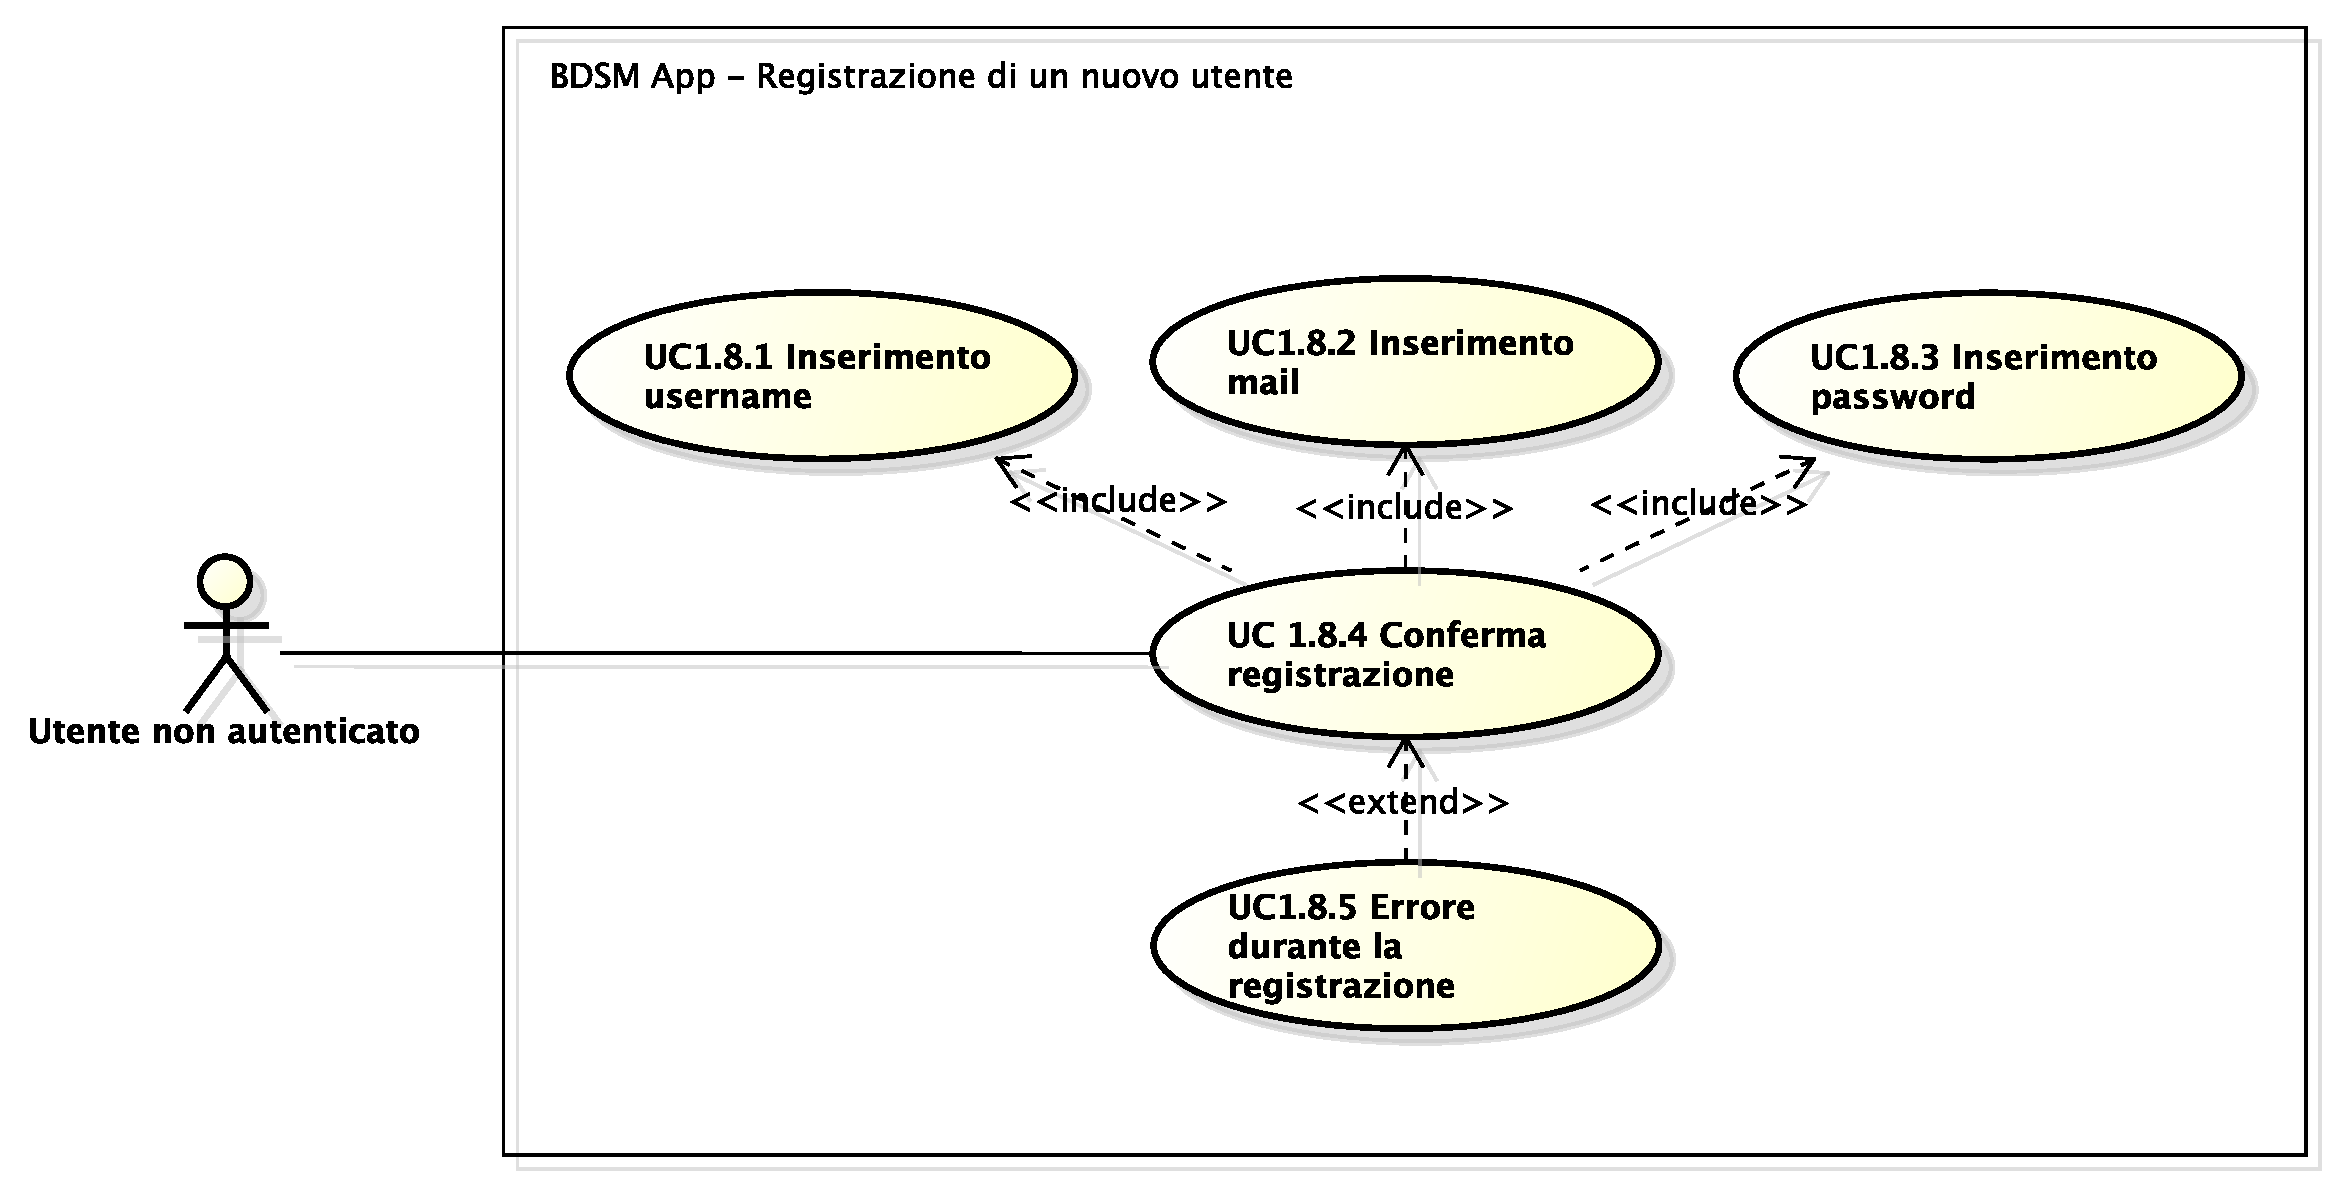
\includegraphics[scale=0.45]{./images/UC1_8.pdf}}
    \caption{Use Case 1.8 - Registrazione di un nuovo utente}
\end{figure}

\begin{itemize}
    \item \textbf{Attori:} Utente
    \item \textbf{Descrizione:} un utente deve poter creare un account per poter eseguire il login
    all’interno del sistema e usufruire delle funzionalità offerte.
    \item \textbf{Precondizione:} l'utente accede al sito web tramite un browser supportato
    dal sistema.
    \item \textbf{Postcondizione:} il sistema ha memorizzato i dati relativi all’account utente e
    ripresenta a questi la schermata iniziale.
    \item \textbf{Flusso principale degli eventi:}

    \begin{enumerate}
        \item inserimento username (UC 1.8.1);
        \item inserimento email (UC 1.8.2);
        \item inserimento password (UC 1.8.3);
        \item conferma registrazione (UC 1.8.4).
        \item errore durante la registrazione (UC 1.8.5)
    \end{enumerate}

\end{itemize}


\subsubsection{UC 1.8.1: Inserimento username}

\begin{itemize}
    \item \textbf{Attori:} Utente
    \item \textbf{Descrizione:} l'utente deve inserire il proprio nome utente per essere riconoscibile univocamente all'interno del sistema e per poter gestire le proprie View.
    \item \textbf{Precondizione:} il sistema fornisce una schermata in cui è possibile inserire l'username per il nuovo account.
    \item \textbf{Postcondizione:} l'utente ha inserito il proprio username.
\end{itemize}

\subsubsection{UC 1.8.2: Inserimento mail}

\begin{itemize}
    \item \textbf{Attori:} Utente
    \item \textbf{Descrizione:}
    \item \textbf{Precondizione:} il sistema fornisce una schermata in cui è possibile inserire la mail per il nuovo account.
    \item \textbf{Postcondizione:} l'utente ha inserito il proprio indirizzo mail.
\end{itemize}

\subsubsection{UC 1.8.3: Inserimento password}

\begin{itemize}
    \item \textbf{Attori:} Utente
    \item \textbf{Descrizione:}
    \item \textbf{Precondizione:} il sistema fornisce una schermata in cui è possibile inserire la password per il nuovo account.
    \item \textbf{Postcondizione:} l'utente ha inserito la password.
\end{itemize}

\subsubsection{UC 1.8.4: Conferma registrazione}

\begin{itemize}
    \item \textbf{Attori:} Utente
    \item \textbf{Descrizione:} l'utente deve poter confermare i dati inseriti durante la registrazione.
    \item \textbf{Precondizione:} il sistema fornisce una schermata in cui è possibile confermare i dati inseriti in precedenza per la creazione di un nuovo account.
    \item \textbf{Postcondizione:} l'utente ha confermato di voler creare un nuovo account all'interno
    del sistema.
\end{itemize}

\subsubsection{UC 1.8.5: Errore durante la registrazione}

\begin{itemize}
    \item \textbf{Attori:} Utente
    \item \textbf{Descrizione:} se vengono inseriti dei dati non conformi ai vincoli di sistema indicati durante la registrazione viene visualizzata una schermata di errore.
    \item \textbf{Precondizione:} i dati inseriti non rispettano uno o più vincoli di sistema.
    \item \textbf{Postcondizione:} l'utente ha visualizzato l'errore relativo ai dati inseriti.
\end{itemize}
